
\begin{table*}[t]
    \centering
    \small
    \setlength{\tabcolsep}{7.5pt}
    \begin{tabular}{ll|ccccccccc|c}
        \toprule
        & Method  & \texttt{360} & \texttt{desk} & \texttt{desk2} & \texttt{floor}& \texttt{plant} & \texttt{room} & \texttt{rpy} & \texttt{teddy} & \texttt{xyz} & \textbf{Avg.} \\
        \midrule

        \cellcolor[HTML]{EEEEEE} & \lo ORB-SLAM3~\cite{campos2021orb}
        & \lo $\times$ & \lo 0.017 & \lo 0.210 & \lo $\times$ & \lo 0.034 & \lo $\times$ & \lo $\times$ & \lo $\times$ & \lo \textbf{0.009} & \lo {N/A} \\
        \cellcolor[HTML]{EEEEEE} & \lo DPV-SLAM~\cite{lipson2024dpvslam}
        & \lo 0.112 & \lo 0.018 & \lo 0.029 & \lo 0.057 & \lo 0.021 & \lo 0.330 & \lo 0.030 & \lo 0.084 & \lo 0.010 & \lo 0.076 \\
        \cellcolor[HTML]{EEEEEE} & \lo DPV-SLAM++~\cite{lipson2024dpvslam}
        & \lo 0.132 & \lo 0.018 & \lo 0.029 & \lo 0.050 & \lo 0.022 & \lo 0.096 & \lo 0.032 & \lo 0.098 & \lo 0.010 & \lo 0.054 \\
        \cellcolor[HTML]{EEEEEE} & \lo DROID-SLAM~\cite{teed2021droid}
        & \lo \textbf{0.111} & \lo 0.018 & \lo 0.042 & \lo \textbf{0.021} & \lo \textbf{0.016} & \lo 0.049 & \lo 0.026 & \lo 0.048 & \lo 0.012 & \lo 0.038 \\
        \multirow{-5}{*}{\cellcolor[HTML]{EEEEEE}\rotatebox[origin=c]{90}{\textit{Calibrated}}}  & \lo GlORIE-SLAM~\cite{zhang2024glorie}
        & \lo 0.128 & \lo \textbf{0.016} & \lo \textbf{0.028} & \lo \textbf{0.021} & \lo 0.021 & \lo \textbf{0.042} & \lo \textbf{0.020} & \lo \textbf{0.035} & \lo 0.010 & \lo \textbf{0.036} \\
        \midrule

        \cellcolor[HTML]{EEEEEE} & CUT3R~\cite{wang2025cut3r}
        & 0.174 & 0.592 & 0.546 & 0.662 & 0.467 & 0.911 & 0.051 & 0.845 & \rd 0.129 & 0.486  \\
        \cellcolor[HTML]{EEEEEE} & SLAM3R~\cite{liu2025slam3r}
        & 0.211 & 0.861 & 0.967 & 0.790 & 0.755 & 1.013 & 0.063 & 0.986 & 0.185 & 0.648 \\
        \cellcolor[HTML]{EEEEEE} & MASt3R-SLAM~\cite{murai2025mast3rslam}
        & \nd 0.070 & \rd 0.032 & \rd 0.055 & \st 0.056 & \nd 0.035 & \nd 0.118 & \rd 0.041 & \rd 0.116 & \nd 0.020 & \nd 0.060 \\
        \cellcolor[HTML]{EEEEEE} & VGGT-SLAM~\cite{maggio2025vggtslam}
        & \st 0.063 & \nd 0.031 & \nd 0.048 & \rd 0.152 & \st 0.023 & \rd 0.133 & \nd 0.038 & \st 0.039 & \nd 0.020 & \rd 0.061 \\
        \multirow{-5}{*}{\cellcolor[HTML]{EEEEEE}\rotatebox[origin=c]{90}{\textit{Uncalibrated}}} & \textbf{\ours}
        & \rd 0.104 & \st 0.030 & \st 0.030 & \nd 0.070 & \rd 0.052 & \st 0.067 & \st 0.023 & \nd 0.080 & \st 0.015 & \st 0.052 \\
        \bottomrule
    \end{tabular}
    \caption{
        \textbf{Camera Trajectory Estimation (ATE RMSE) on TUM-RGBD~\cite{sturm12tumrgbd}.}
        \ours performs the best on average.
    }
    \label{tab:traj_tumrgbd}
    \vspace{-0.5em}
\end{table*}

\vspace{-0.1em}
\section{Experiments}
\vspace{-0.1em}
\label{sec:exp}
% \subsection{Experimental setup}
% \boldparagraph{Evaluation Datasets and Metric}
% We follow the evaluation protocol of VGGT-SLAM~\cite{maggio2025vggtslam} and test \ours on standard monocular SLAM benchmarks to assess both camera tracking accuracy and reconstruction quality. Specifically, we report the \textit{root mean square error (RMSE) of the absolute trajectory error (ATE)} (unit: m) on the real-world datasets 7-Scenes~\cite{shotton2013-7scenes} and TUM-RGBD~\cite{sturm12tumrgbd}, using the evo toolkit~\cite{grupp2017evo}. To evaluate the quality of scene reconstruction, we measure \textit{RMSE} of \textit{accuracy}, \textit{completion}, and \textit{Chamfer distance} (unit: m) on the 7-Scenes dataset, which provides ground-truth 3D scenes.

\boldparagraph{Evaluation Datasets and Metrics}
Following VGGT-SLAM~\cite{maggio2025vggtslam}, we evaluate our method on standard monocular SLAM benchmarks for camera tracking accuracy and reconstruction quality. We report root mean square error (RMSE) of absolute trajectory error (ATE, in meters) on real-world 7-Scenes~\cite{shotton2013-7scenes} and TUM-RGBD~\cite{sturm12tumrgbd} datasets using the evo toolkit~\cite{grupp2017evo}. Reconstruction quality on 7-Scenes is assessed via RMSE of accuracy, completion, and Chamfer distance (meters), leveraging its ground-truth 3D scenes.

\boldparagraph{Implementation Details}
The frontend STA model is initialized from the weights of DUSt3R~\cite{dust3r}, and trained on  ScanNet~\cite{dai2017scannet}, ScanNet++\cite{yeshwanthliu2023scannetpp}, ARKitScenes\cite{dehghan2021arkitscenes}, CO3D~\cite{reizenstein21co3d}, Aria Synthetic Environments~\cite{avetisyan2024ase}, and Replica~\cite{replica19arxiv} for 7 days using 8 NVIDIA H100 GPUs.
We use AdamW optimizer to train our STA model with learning rate $1.5e^{-5}$, weight decay $0.01$, $B=12$, $\alpha^{\text{point}}=0.2$, $\alpha^{\text{pose}}=0.05$, $\lambda_{\text{pmap}}=1$, $\lambda_{\text{pose}}=1$, $\lambda_{\text{gc}}=1$, and $\tau_p = 0.75$. We conducted evaluations on a machine with an NVIDIA RTX 4090 GPU and an Intel i9-14900KF CPU, with $N=2$ for 7-Scenes and $N=3$ for TUM-RGBD.

% machine: atcremers122

\boldparagraph{Baselines}
\ours is primarily compared with state-of-the-art (SOTA) learning-based SLAM methods in uncalibrated scenarios: VGGT-SLAM~\cite{maggio2025vggtslam}, MASt3R-SLAM~\cite{murai2025mast3rslam}, SLAM3R~\cite{liu2025slam3r}, and CUT3R~\cite{wang2025cut3r}. To reduce randomness from VGGT-SLAM’s RANSAC, we run it 5 times per scene as suggested in their paper; results for other methods, including ours, are deterministic. We also compare with SOTA methods using known camera intrinsics~\cite{campos2021orb,zhu2024nicer,zhang2024glorie,teed2021droid,lipson2024dpvslam}. Some results are taken from~\cite{murai2025mast3rslam,maggio2025vggtslam}. For MASt3R-SLAM and VGGT-SLAM, we keep their original keyframe selection; for ours, CUT3R, and SLAM3R, we use frame strides of 5 (7-Scenes) and 3 (TUM-RGBD). Calibrated methods are shown in {\lo gray}. Best results are highlighted as \colorbox{colorFst}{\bf first}, \colorbox{colorSnd}{second}, and \colorbox{colorTrd}{third}.

\subsection{Camera Trajectory Evaluation}
\label{subsec:traj}



In \cref{tab:traj_7scenes} and \cref{tab:traj_tumrgbd}, we report ATE RMSE. \ours achieves the best average performance on both datasets, outperforming current SOTA~\cite{murai2025mast3rslam} by 17\% (0.055 vs. 0.066) and 13\% (0.052 vs. 0.060), and surpasses some calibrated methods~\cite{zhu2024nicer,lipson2024dpvslam}. \ours performs less effectively on TUM-RGBD  \texttt{360} scene due to predominantly rotational camera motion that leads to frontend ambiguity and degrading performance.
% Other methods~\cite{murai2025mast3rslam,maggio2025vggtslam} address this using multi-view frontends or bundle adjustment.
Other methods~\cite{murai2025mast3rslam,maggio2025vggtslam} use either heavier multi-view frontend or more intensive optimization to reduce the influence.
Pure regression-based methods~\cite{wang2025cut3r,liu2025slam3r} struggle to maintain consistent registration over long sequences with large camera motion due to forgetting effects.

In \cref{fig:traj}, we show the estimated trajectories from different methods on 7-Scenes~\cite{shotton2013-7scenes} \texttt{office} and TUM-RGBD~\cite{sturm12tumrgbd} \texttt{room}. CUT3R~\cite{wang2025cut3r} suffers from severe forgetting issues on long sequences; SLAM3R~\cite{liu2025slam3r} has bad point registration on the challenged scene TUM-RGBD \texttt{room}, thus, does not produce correct camera poses. Compared to pure regression-based methods, MASt3R-SLAM~\cite{murai2025mast3rslam} and VGGT-SLAM~\cite{maggio2025vggtslam} work well, while \ours achieves even higher trajectory accuracy.


\begin{figure*}[!htb]
\centering
{\footnotesize
    \setlength{\tabcolsep}{0pt}
    \renewcommand{\arraystretch}{1}
    \newcommand{\sz}{1}
    \begin{tabular}{c}
        % 7-Scenes \texttt{office} \\
      \vspace{-1em}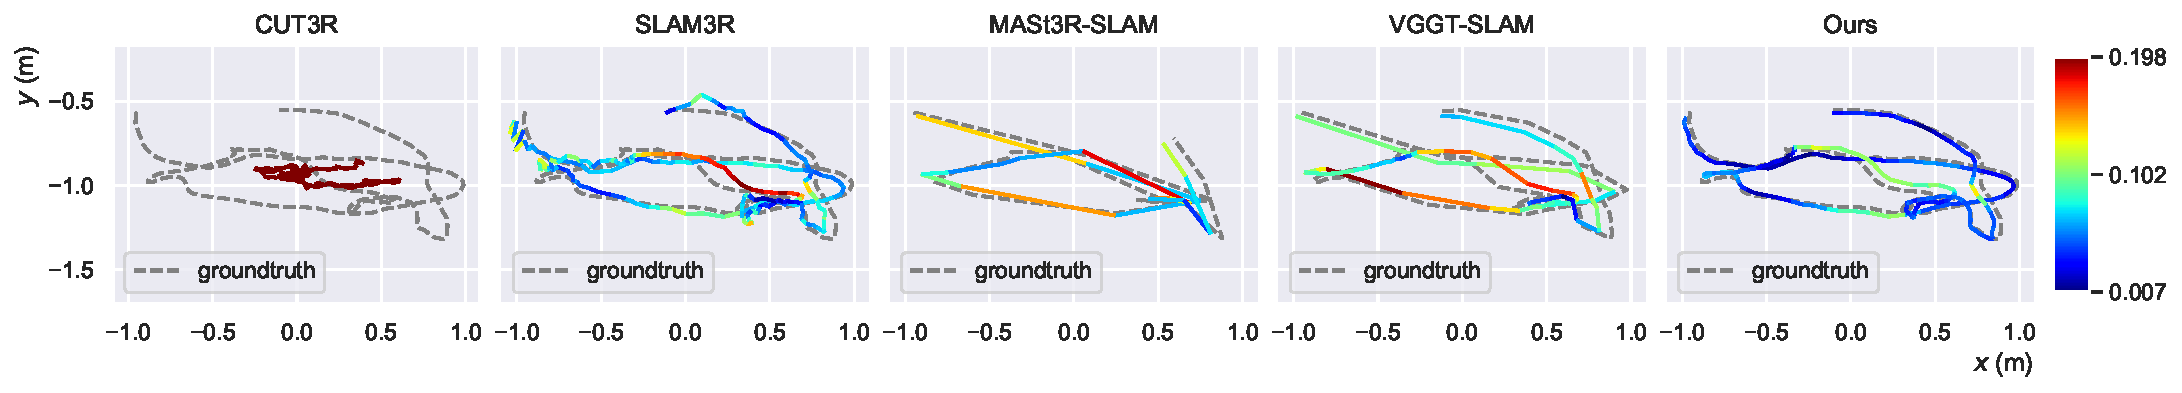
\includegraphics[width=\sz\linewidth]{figs/traj/traj_plot_7scenes.pdf} \\ [-12pt]
     % TUM-RGBD \texttt{room} \\
     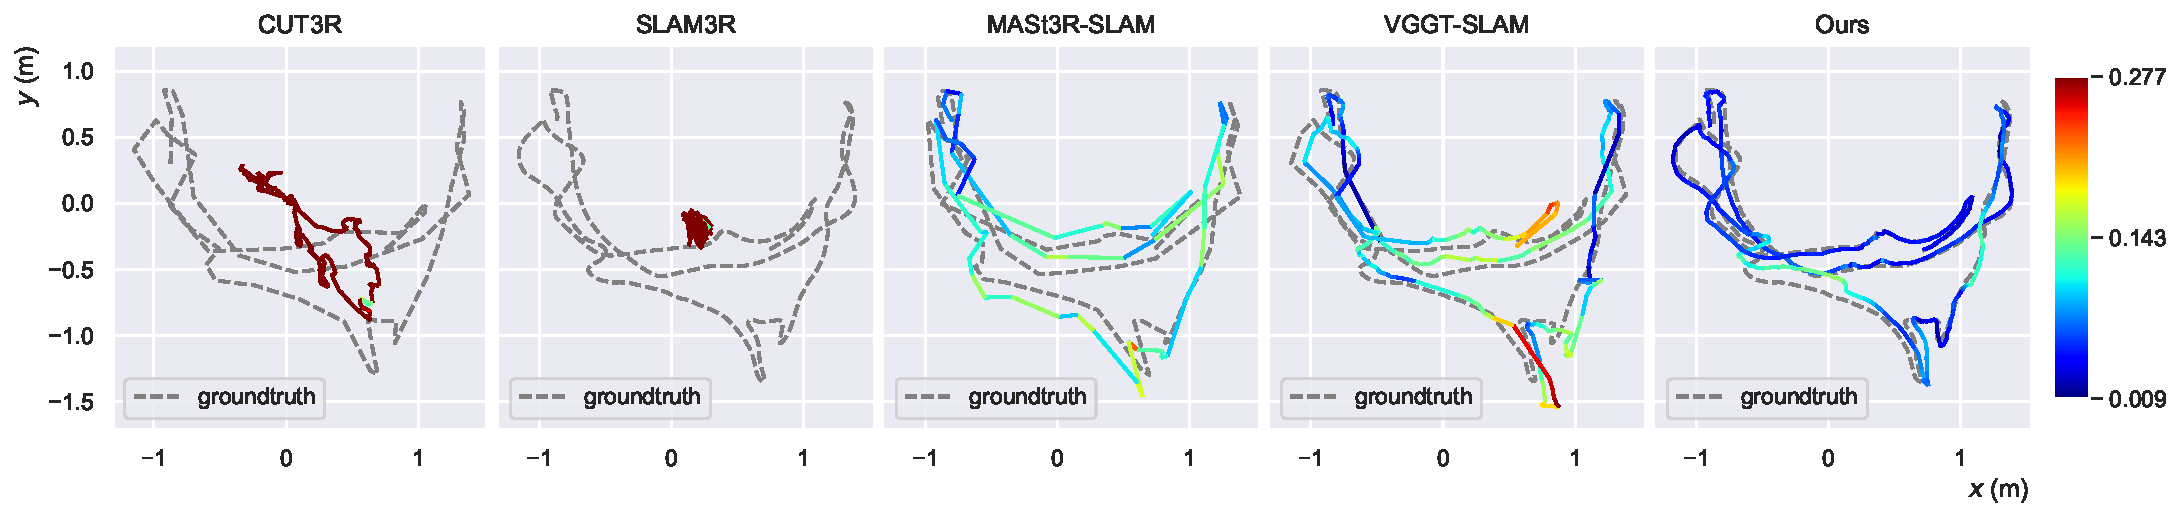
\includegraphics[width=\sz\linewidth]{figs/traj/traj_plot_tumrgbd.pdf} \\ [-8pt]


    \end{tabular}
}

\caption{\textbf{Trajectory estimation results on 7-Scenes \texttt{office} (top) and TUM-RGBD \texttt{room} (bottom).}
Estimated camera trajectories are projected onto the $x$–$y$ plane, with ground-truth shown as dashed lines. The trajectory color encodes ATE RMSE: higher errors in red, lower in blue. For MASt3R-SLAM~\cite{murai2025mast3rslam} and VGGT-SLAM~\cite{maggio2025vggtslam}, only the poses of their selected keyframes are estimated.}

\label{fig:traj}
\vspace{-1em}
\end{figure*}


\subsection{Dense Reconstruction Evaluation}

\label{subsec:recon}

\begin{table}[t]
    \centering
    \vspace{0.5em}
    % \scriptsize
    \small
    \setlength{\tabcolsep}{4pt}
    \resizebox{\columnwidth}{!}
    {
    \begin{tabular}{l|c|ccc}
    \toprule
    Method  & ATE $\downarrow$ & Acc. $\downarrow$ & Comp. $\downarrow$ & Chamfer $\downarrow$\\
    \midrule
    \lo DROID-SLAM~\cite{teed2021droid}
    &\lo 0.049 &\lo 0.141 &\lo\bf 0.048 &\lo 0.094\\
    \lo MASt3R-SLAM~\cite{murai2025mast3rslam}
     &\lo\bf0.047 &\lo\bf 0.089 &\lo 0.085 &\lo\bf 0.087\\
    \midrule
    Spann3R @20~\cite{wang2025spann3r}
    & N/A & 0.069 & \nd 0.047 & 0.058\\
    Spann3R @2~\cite{wang2025spann3r}
    & N/A & 0.124 & \st 0.043 & 0.084\\
    CUT3R~\cite{wang2025cut3r}
    & 0.477 & 0.276 & 0.303 & 0.290\\
    SLAM3R~\cite{liu2025slam3r}
    & 0.098 & 0.053 & 0.059 & \nd 0.056\\
    MASt3R-SLAM~\cite{murai2025mast3rslam}
    &\rd 0.066  & 0.059 & \rd 0.056 & \rd 0.057\\
    VGGT-SLAM~\cite{maggio2025vggtslam}
    &  0.070  & \rd 0.052 & 0.060 & \nd 0.056\\
    2-view VGGT \emph{w/} PGO
    &\nd 0.065 & \st 0.039 & 0.077 & 0.058\\
    \textbf{\ours}
    & \st 0.055  & \nd 0.045 & \rd 0.056 & \st 0.051\\
    \bottomrule
    \end{tabular}
    }
    \caption{
    \textbf{Tracking and Reconstruction Evaluation on 7-Scenes~\cite{shotton2013-7scenes}.} @$n$ indicates a keyframe every $n$ images. \textit{2-view VGGT w/ PGO} uses the 2-view VGGT frontend with the same pose graph optimization as ours. \ours achieves the best trajectory estimation and reconstruction performance on 7-Scenes.
    % Our method performs on average competitively with HI-SLAM and better than all other methods. Results for the RGB-D methods are from \cite{liso2024loopyslam}.
    }
    \label{tab:recon_7scenes}
    \vspace{2em}

    % \vspace{-0pt}  % move closer to prev. table
    \centering
    % \scriptsize
    % \footnotesize
    \small
    \setlength{\tabcolsep}{3pt}
    \resizebox{\columnwidth}{!}
    {
    \begin{tabular}{lcccccc}
    \toprule
      & CUT3R & SLAM3R
      % & GlORIE-$\textcolor{red}{^*}$
      & MASt3R & VGGT &  2-view VGGT & \bf \ourshort\\
      & \cite{wang2025cut3r} & \cite{liu2025slam3r}& SLAM~\cite{murai2025mast3rslam} & SLAM~\cite{maggio2025vggtslam}& \emph{w/} PGO &\bf SLAM\\
    \midrule
    Size $\downarrow$ & 0.79 & \rd 0.76 & \nd 0.69 & 1.26 & 1.26 & \st0.44\\[2pt] \hdashline \noalign{\vskip 2pt}
    FPS $\uparrow$ & 34.2 & \rd 45.8 &30.3 & \st 93.3 & 12.6 & \nd 78.0\\
    \bottomrule
    \end{tabular}
    }
    % \vspace{2pt}
    \caption{
        \textbf{Model Size and Running Time Evaluation on 7-Scenes~\cite{shotton2013-7scenes} \texttt{redkitchen}.} Model sizes are reported in billions of parameters. FPS indicates the average number of frames processed per second over three runs. \ours shows highly competitive real-time speed with the smallest model size among baselines.
    }
    \label{tab:size_and_time}
    \vspace{-1em}

\end{table}




% In \cref{tab:recon_7scenes}, we evaluate reconstruction quality across methods. Leveraging accurate camera poses and consistent local pointclouds, \ours achieves the best Chamfer distance among all approaches. Despite using a lightweight two-view frontend, \ours, combined with a tailored $\mathrm{Sim}(3)$ pose graph optimization and loop closure, significantly outperforms multiview-based methods~\cite{liu2025slam3r,maggio2025vggtslam} in accuracy (0.45 vs. 0.52) while matching or exceeding their completeness.
% We also test the 2-view version of VGGT with the same pose graph optimization as ours, while the accuracy is comparable, our method performs better overall, demonstrating the effectiveness of our lightweight frontend.

In \cref{tab:recon_7scenes}, we evaluate reconstruction quality across methods. Leveraging accurate camera poses and consistent local point clouds, \ours achieves the best Chamfer distance among all approaches. Despite using a lightweight two-view frontend, \ours, combined with tailored $\mathrm{Sim}(3)$ pose graph optimization, significantly outperforms multi-view-frontend methods~\cite{liu2025slam3r,maggio2025vggtslam} in accuracy (0.45 vs. 0.52) while matching or exceeding completeness.
To demonstrate the effectiveness of our lightweight frontend, we add another strong baseline, replacing our STA model with a two-view VGGT~\cite{wang2025vggt} as the frontend and conducting the same pose graph optimization. \ours still achieves better performance in Chamfer distance, completeness, and absolute trajectory error, highlighting the effectiveness of our lightweight symmetric frontend over larger multiview models like VGGT for SLAM tasks



In \cref{fig:recon}, we show qualitative reconstruction results on 7-Scenes \texttt{redkitchen}, TUM-RGBD~\cite{sturm12tumrgbd} \texttt{room}, and BundleFusion~\cite{dai2017bundlefusion} \texttt{apt1}. CUT3R~\cite{wang2025cut3r} fails to reconstruct correctly due to forgetting issues, while SLAM3R~\cite{liu2025slam3r} struggles in scenes with large camera perspective changes. MASt3R-SLAM~\cite{murai2025mast3rslam} and VGGT-SLAM~\cite{maggio2025vggtslam} produce artifacts on object boundaries, failing to clearly separate foreground from background, and show misalignment across views. In contrast, \ours overcomes these challenges through geometric consistency constraints during training. Notably, VGGT-SLAM fails midway through the \texttt{apt1} scene as backend optimization diverges, which stems from the unstable RANSAC-based 3D homography estimation, which can sample planar regions and cause ambiguity in their proposed $\mathrm{SL}(4)$ pose graph optimization.
\begin{figure*}[!ht]
\centering
{\footnotesize
    \setlength{\tabcolsep}{3pt}
    \renewcommand{\arraystretch}{1}
    \newcommand{\sz}{0.3}
    \begin{tabular}{cccc}
    \rotatebox{90}{\hspace{1.2em} \small \makecell{CUT3R~\cite{wang2025cut3r}}} &
        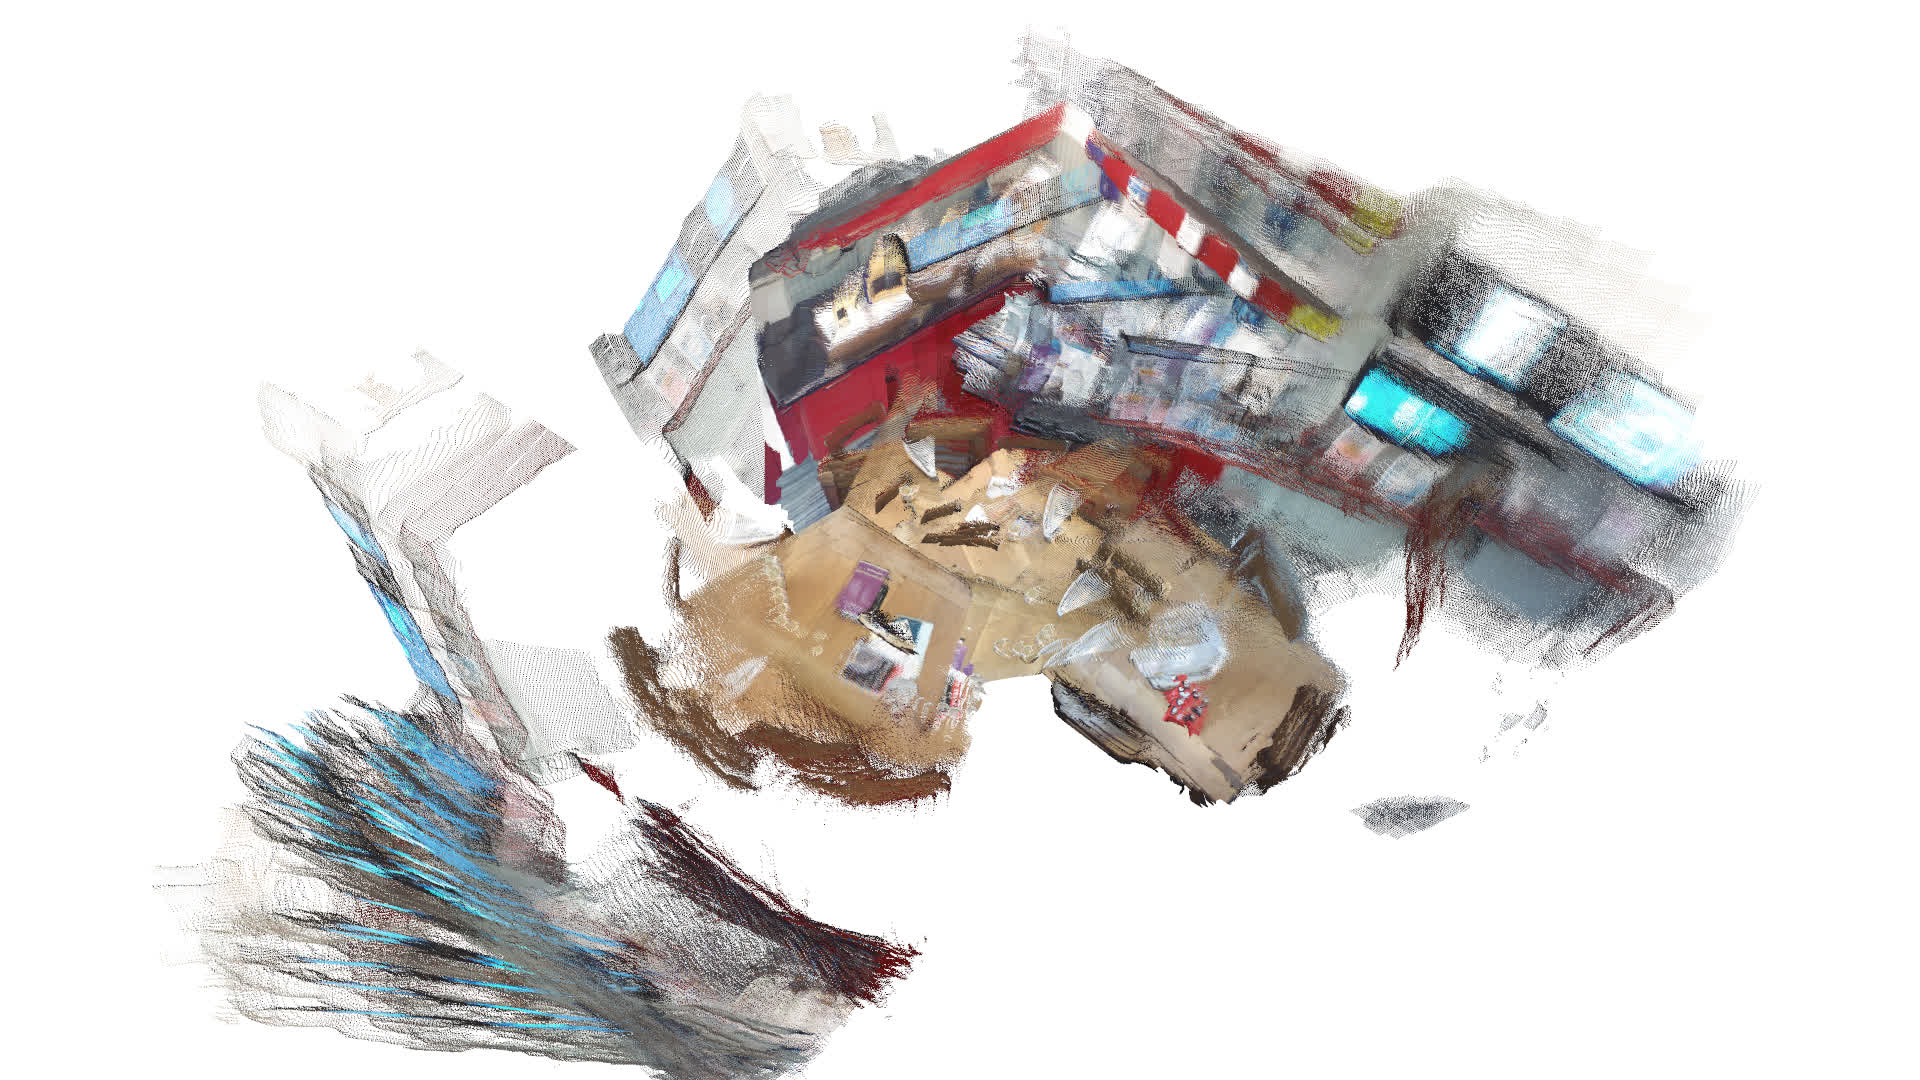
\includegraphics[width=\sz\linewidth]{figs/recon/7scenes_redkitchen_cut3r_screenshot_000.jpg} & 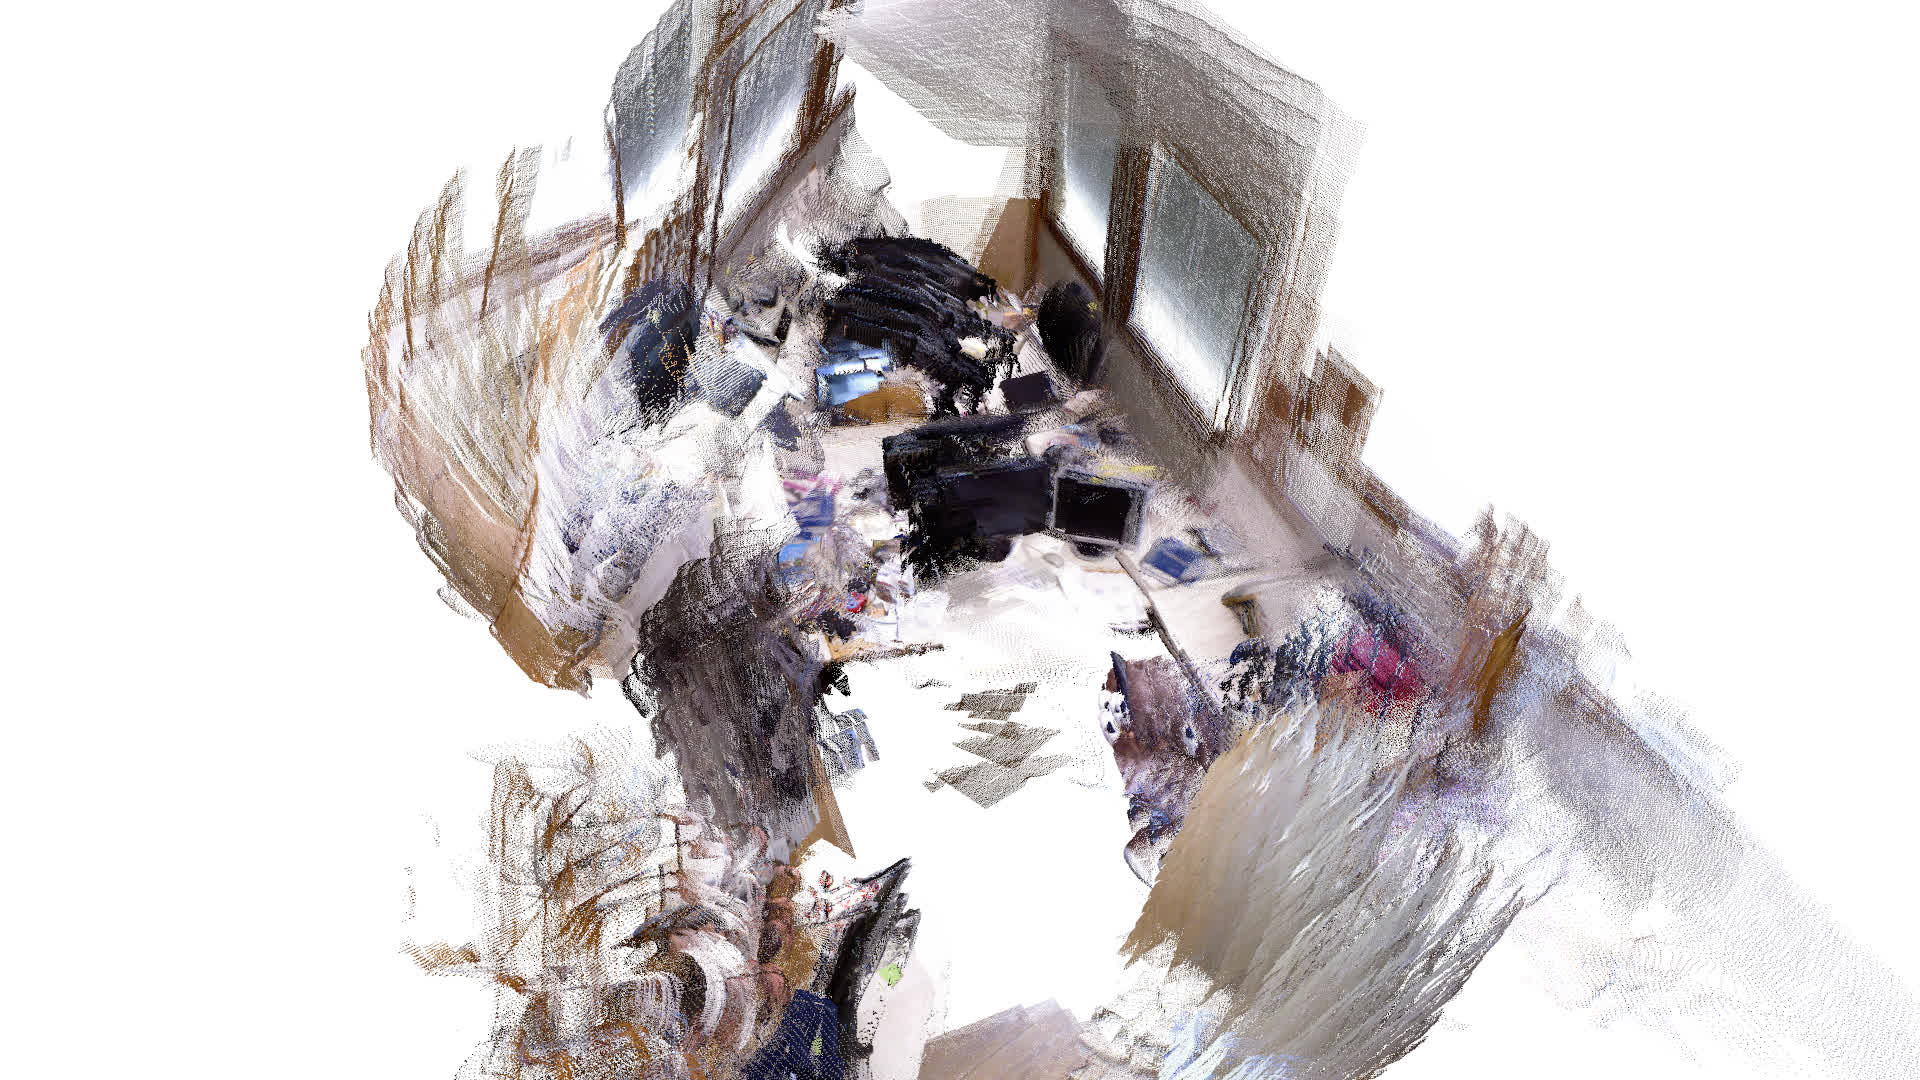
\includegraphics[width=\sz\linewidth]{figs/recon/tumrgbd_room_cut3r_screenshot_000.jpg} &
        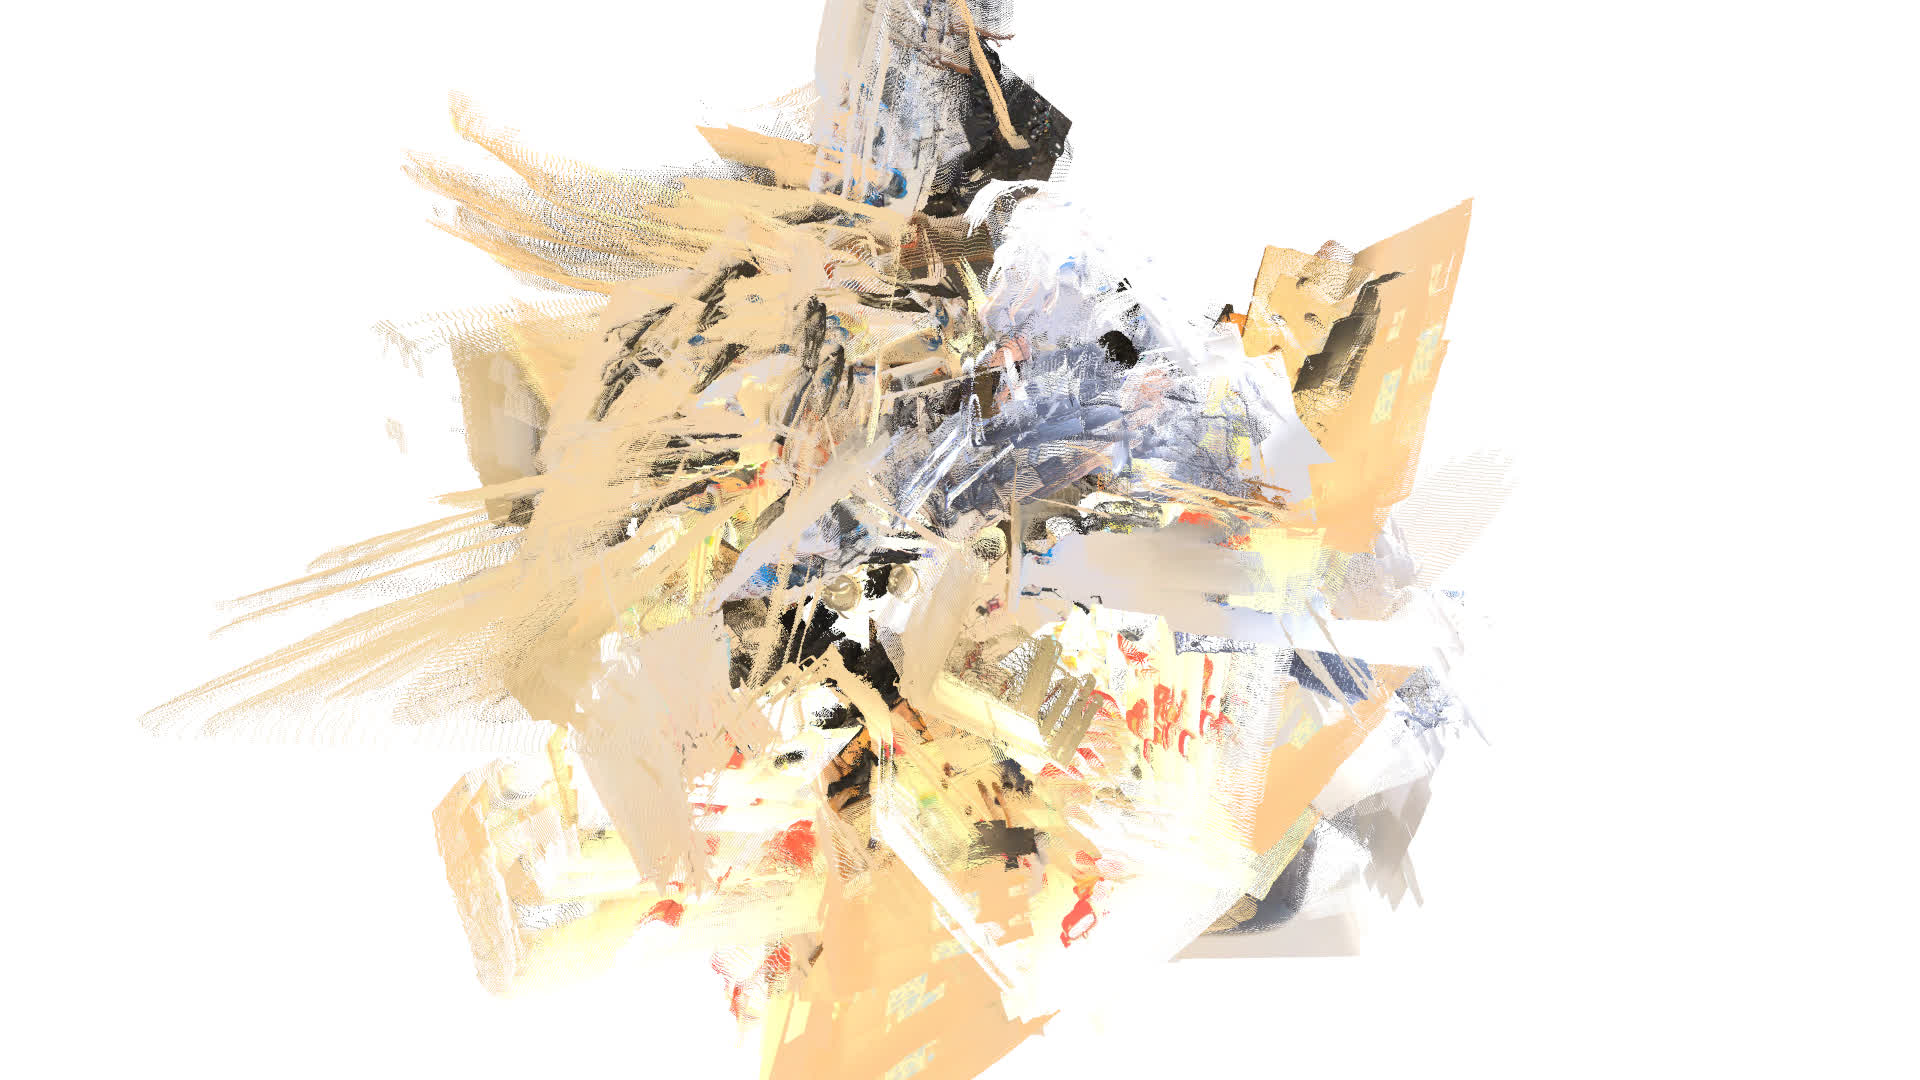
\includegraphics[width=\sz\linewidth]{figs/recon/bf_apt1_cut3r_screenshot_000.jpg}\\
    \rotatebox{90}{\hspace{1.2em} \small \makecell{SLAM3R~\cite{liu2025slam3r}}} &
        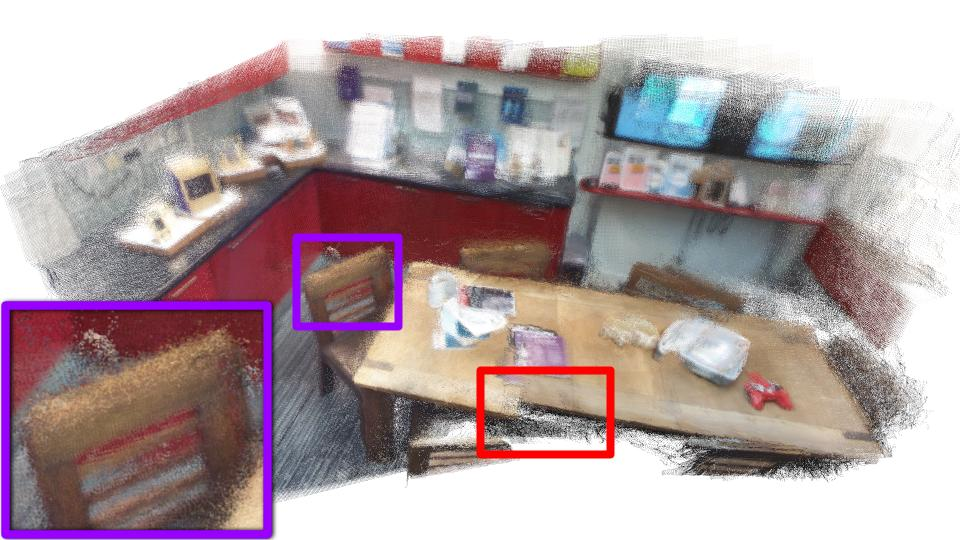
\includegraphics[width=\sz\linewidth]{figs/recon/7scenes_slam3r.jpg} & 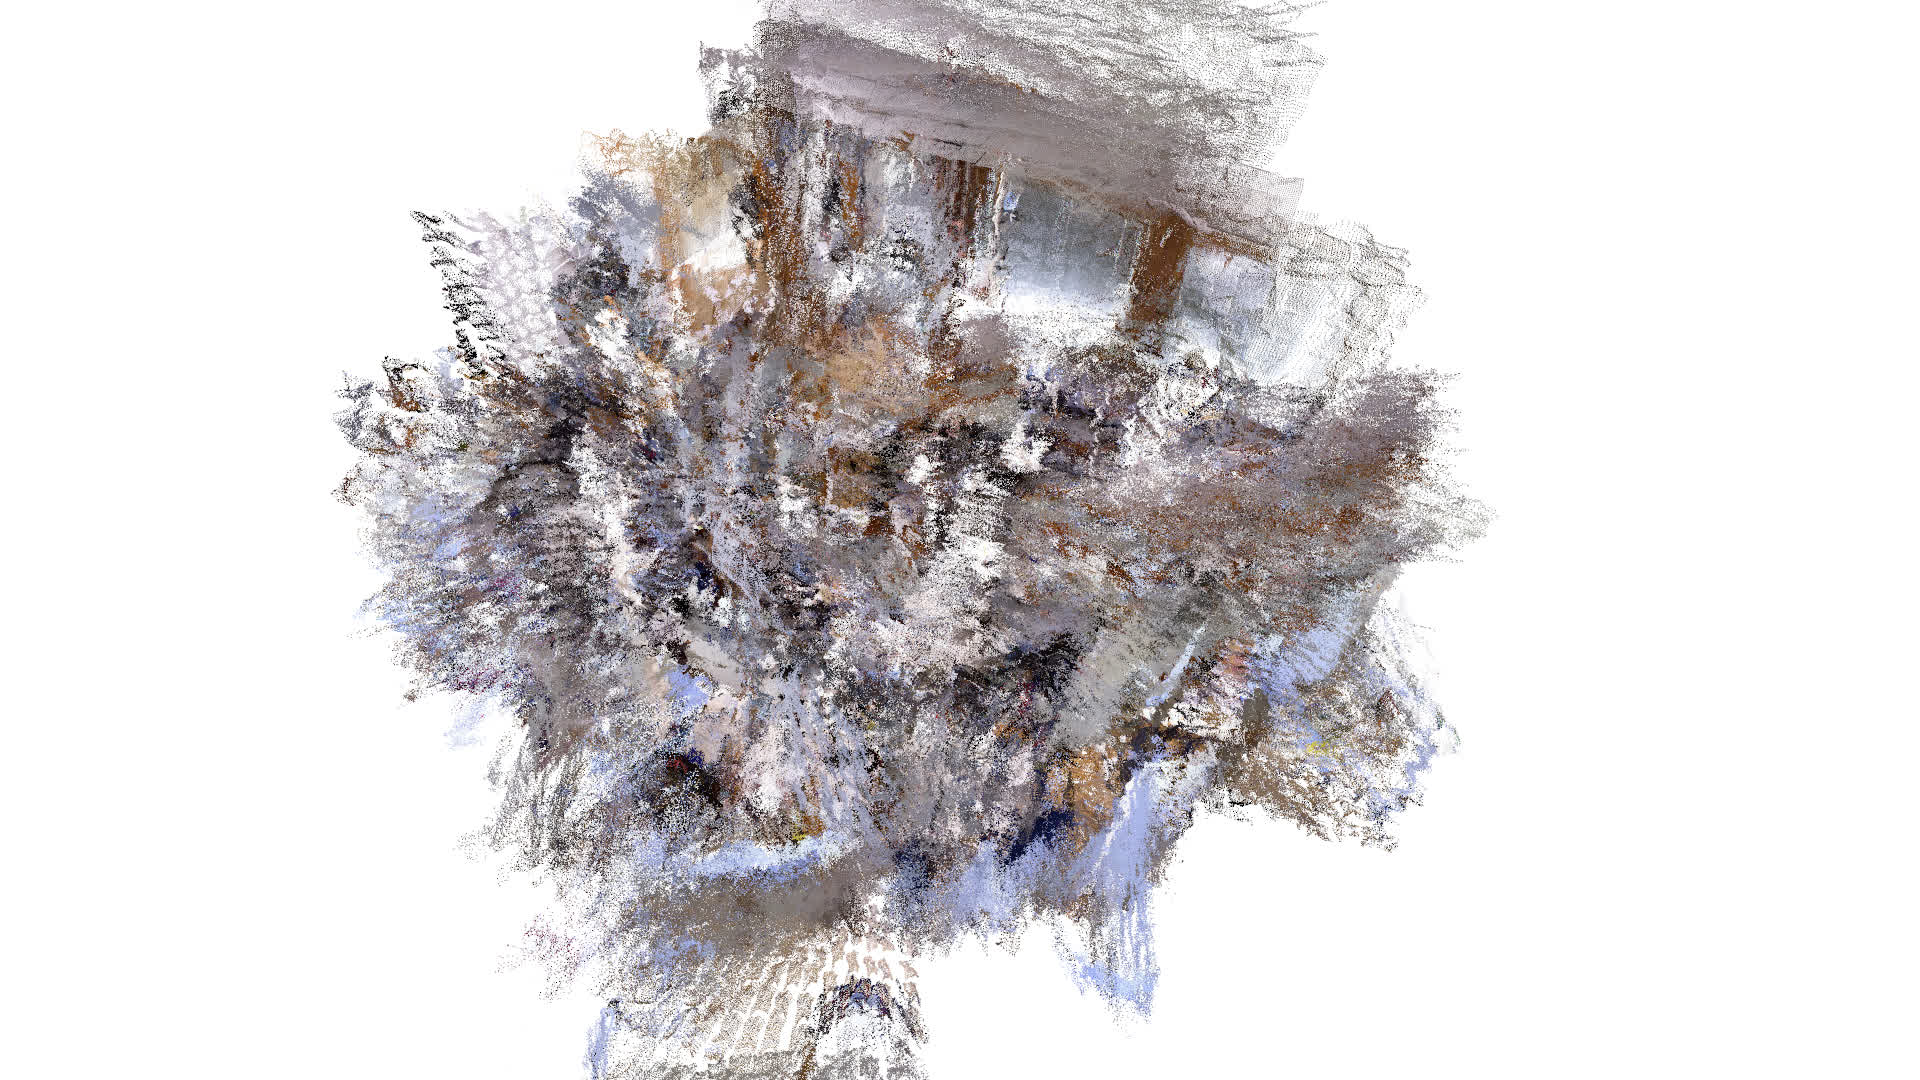
\includegraphics[width=\sz\linewidth]{figs/recon/tumrgbd_room_slam3r_screenshot_000.jpg} &
        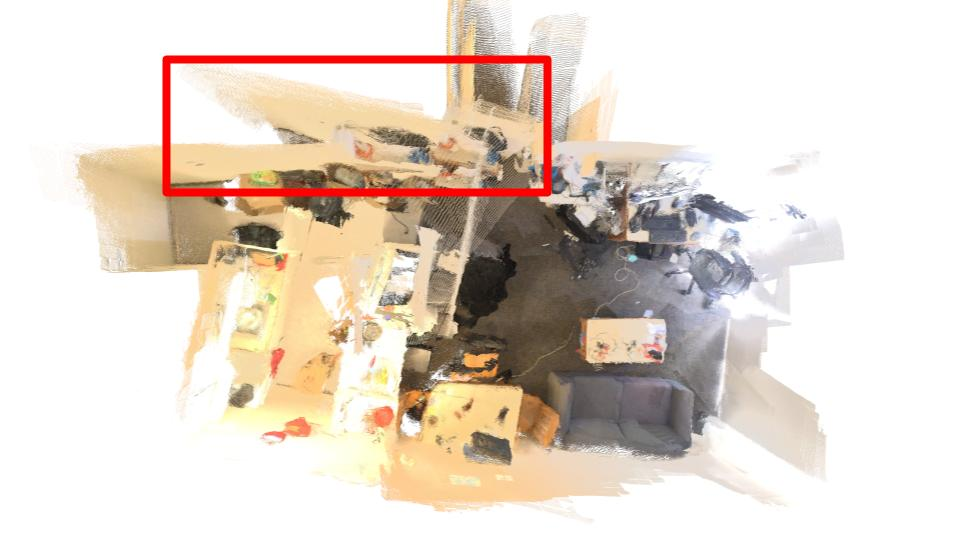
\includegraphics[width=\sz\linewidth]{figs/recon/bf_slam3r.jpg}\\
    \rotatebox{90}{\hspace{1.8em} \small \makecell{MASt3R-\\\hspace{0.5em}SLAM~\cite{murai2025mast3rslam}}} &
        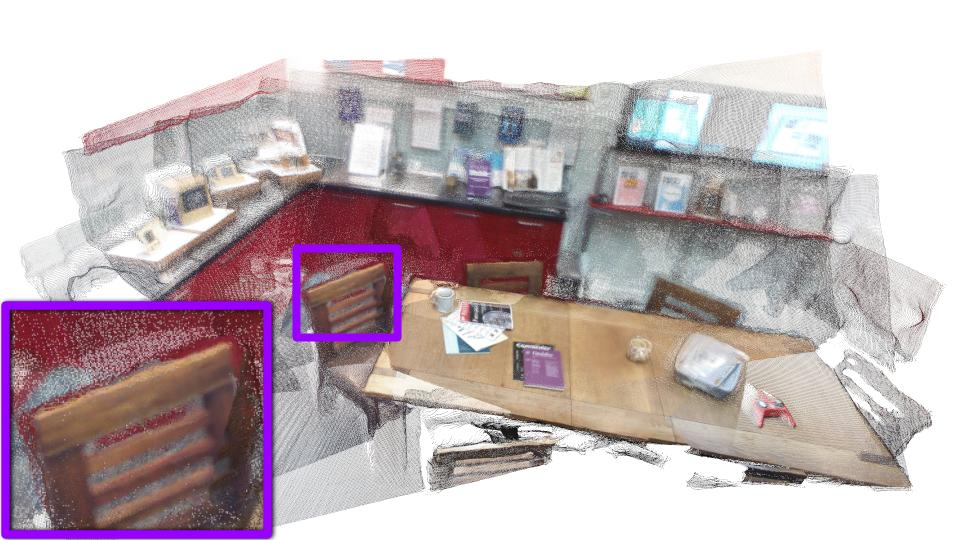
\includegraphics[width=\sz\linewidth]{figs/recon/7scenes_mast3rslam.jpg} & 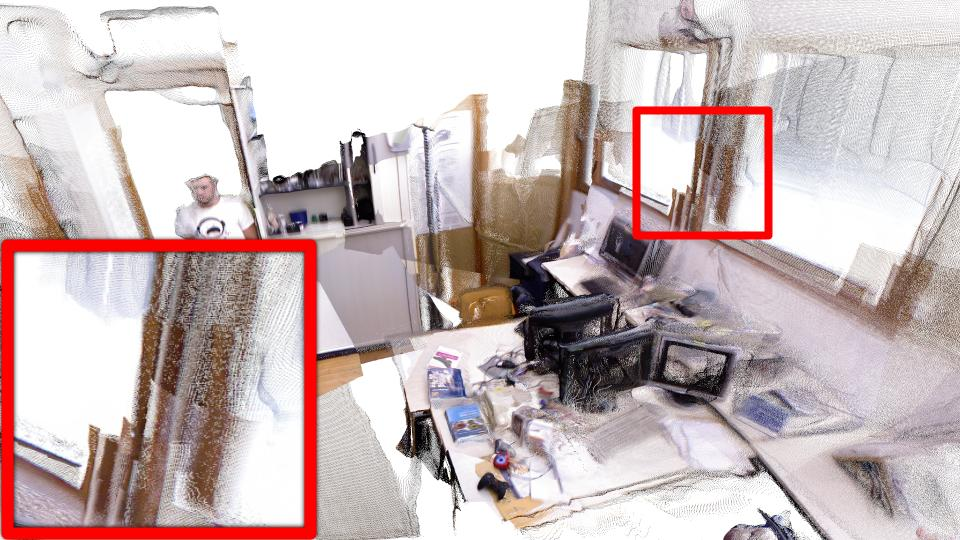
\includegraphics[width=\sz\linewidth]{figs/recon/tum_mast3rslam.jpg} &
        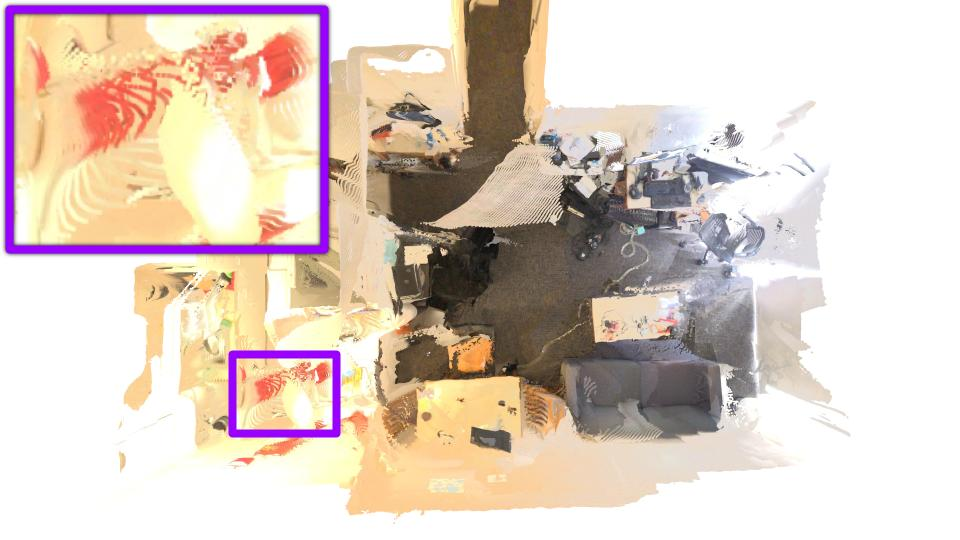
\includegraphics[width=\sz\linewidth]{figs/recon/bf_mast3rslam.jpg}\\
    \rotatebox{90}{\hspace{2.2em} \small \makecell{VGGT-\\\hspace{0.5em}SLAM~\cite{maggio2025vggtslam}}} &
        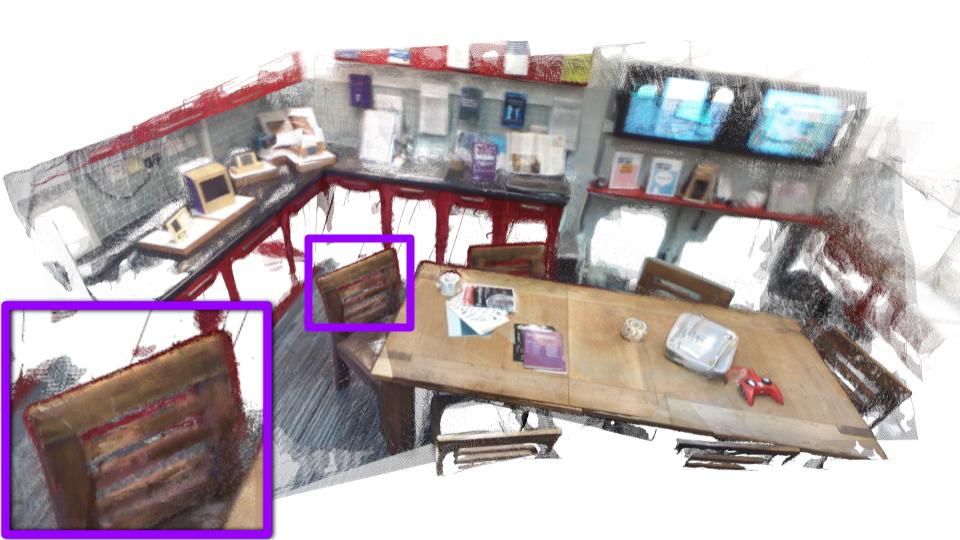
\includegraphics[width=\sz\linewidth]{figs/recon/7scenes_vggtslam.jpg} & 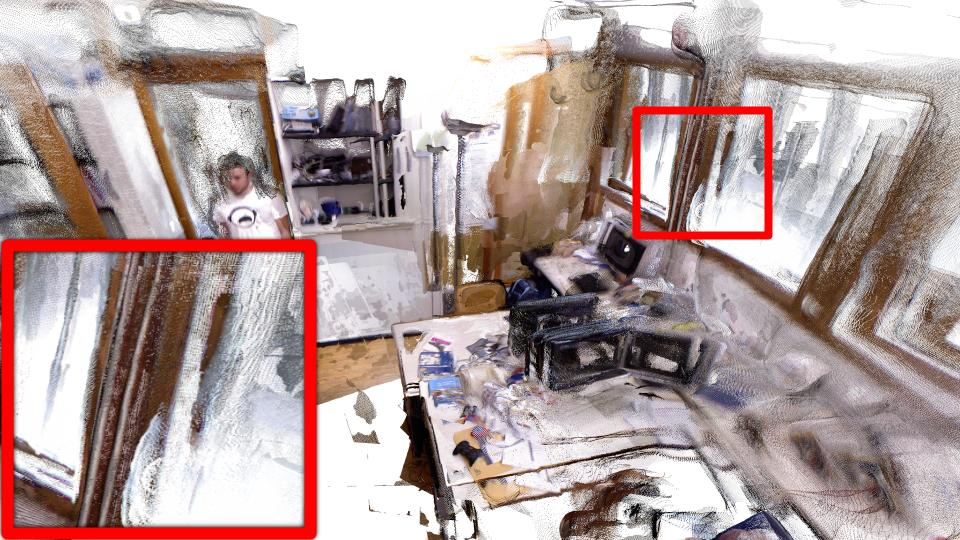
\includegraphics[width=\sz\linewidth]{figs/recon/tum_vggtslam.jpg} &
        
\includegraphics[width=\sz\linewidth]{figs/recon/bf_vggtslam_fail.jpg}\\
    \rotatebox{90}{\hspace{3.2em} \small \makecell{\bf \ours}} &
        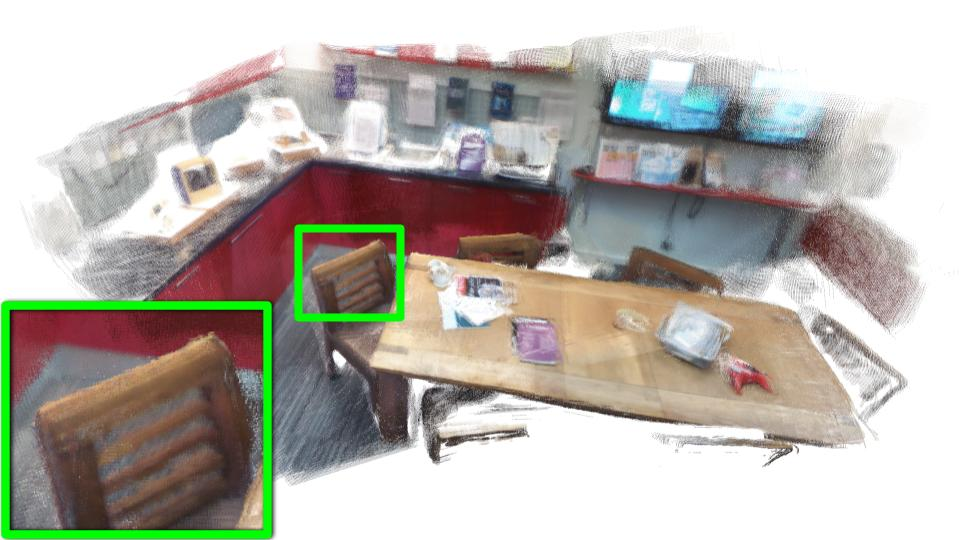
\includegraphics[width=\sz\linewidth]{figs/recon/7scenes_ours.jpg} & 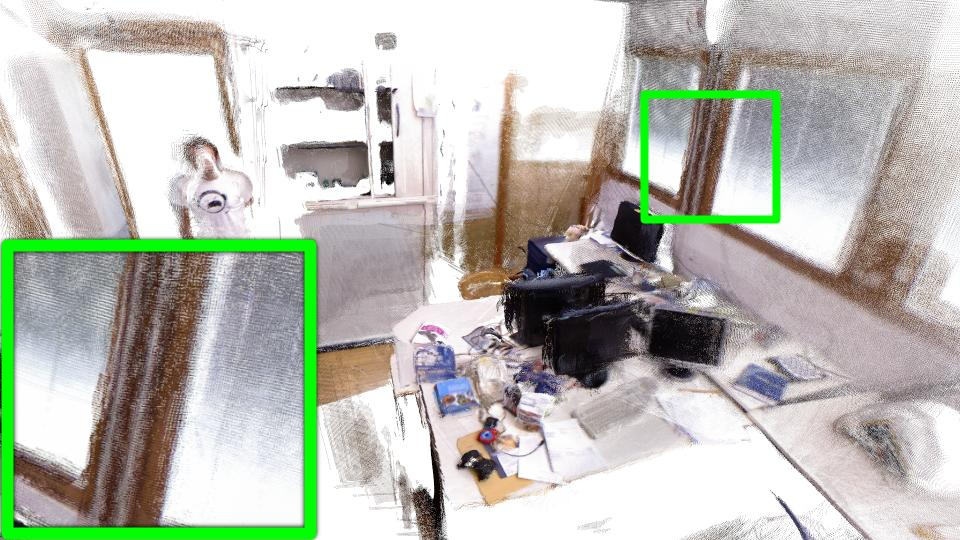
\includegraphics[width=\sz\linewidth]{figs/recon/tum_ours.jpg} &
        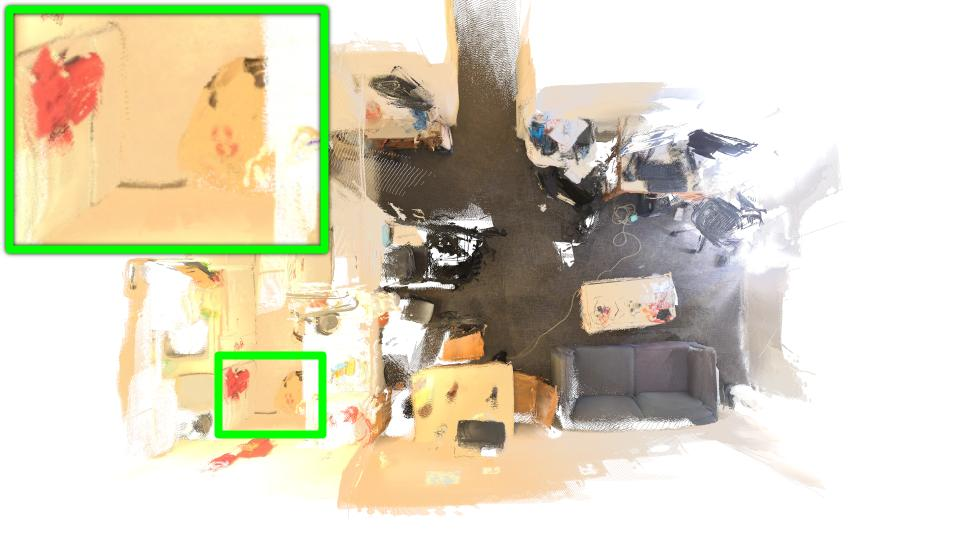
\includegraphics[width=\sz\linewidth]{figs/recon/bf_ours.jpg}\\
    \end{tabular}
}
\caption{\textbf{Reconstruction results on 7-Scenes \texttt{redkitchen} (left), TUM-RGBD \texttt{room} (middle), and BundleFusion \texttt{apt1} (right).}
Purple boxes highlight reconstruction artifacts near the edges (background points wrongly mapped to the edge of the foreground). Red boxes indicate misalignments. Green boxes highlights \ours's competitive results.
VGGT-SLAM fails to complete reconstruction on \texttt{apt1} due to divergence in pose graph optimization.}
\label{fig:recon}
\vspace{-1em}
\end{figure*}





\subsection{Model Size and Speed}
\label{subsec:size_speed}

\begin{table}[t]
    % \vspace{-0pt}  % move closer to prev. table
    \centering
    % \scriptsize
    % \footnotesize
    \small
    \setlength{\tabcolsep}{5pt}
    \resizebox{\columnwidth}{!}
    {
    \begin{tabular}{lcccccc}
    \toprule
      & load & encoder & decoder & detect & construct & optimize
      \\
      & data &  &  & loop & graph & graph\\
    \midrule
    time (s) & 1.88 & 0.89 & 3.38 & 0.41 & 2.93 & 3.31\\
    \% & 14.7\% & 7.0\% & 26.4\% & 3.18\% & 22.9\% & 25.9\% \\
    \bottomrule
    \end{tabular}
    }
    \caption{
        \textbf{Time Spent on Each Component of \ours for 7-Scenes~\cite{shotton2013-7scenes} \texttt{redkitchen} (in seconds and percentage).}
        % There are 1000 frames in this scene.
    }
    \label{tab:step_time}
    \vspace{1em}

    \centering
    \small
    \setlength{\tabcolsep}{7.5pt}
    \begin{tabular}{llcc}
        \toprule
        % \multirow{2}{*}{\multicolumn{2}{c}{Settings}}
        \multicolumn{2}{c}{Settings}& ATE $\downarrow$ & Chamfer $\downarrow$ \\
        \midrule
        % \multicolumn{2}{c}{2-view VGGT + pose graph}  & 0.065 & \rd 0.058 \\
        % \midrule
        \multirow{2}{*}{\textit{STA Model}}
        & \wo $L_\text{gc}$ & \nd 0.056 & \nd 0.057 \\
        & \wo $L_\text{id}$ & 0.058 & \rd 0.059 \\
        \midrule
        \multirow{3}{*}{\textit{Pose Graph}}
        & \wo pose graph opt. & 0.105 & 0.070 \\
        & \wo loop closure & 0.103 & 0.072 \\
        & \wo two edge types & \rd 0.057 & \st 0.051 \\

        \midrule
        \multicolumn{2}{c}{\bf \ours with full features}
             & \st 0.055 & \st 0.051 \\
        \bottomrule
    \end{tabular}

    \caption{
        \textbf{Ablation Study on 7-Scenes~\cite{shotton2013-7scenes}.}
        % \textit{2-view VGGT} here replaces STA model with VGGT (input 2 views each time) as frontend.
        \textit{w/o pose graph opt.} simply accumulates relative poses for absolute poses. \textit{w/o two edge types} uses the classical pose graph in which each view is represented by a single node.
    }
    \label{tab:ablation}
    \vspace{-1.5em}
\end{table}


We compare the frontend model size and processing speed across methods in \cref{tab:size_and_time}. Owing to our symmetric design, the decoder and regression heads use only half the parameters of existing feedforward models~\cite{dust3r,mast3r,wang2025spann3r,liu2025slam3r}. Consequently, our model is far more compact: only 64\% the size of MASt3R~\cite{mast3r} (used in MASt3R-SLAM~\cite{murai2025mast3rslam}) and 35\% the size of VGGT~\cite{wang2025vggt} (used in VGGT-SLAM~\cite{maggio2025vggtslam}).


The speed evaluation further confirms that \ours achieves real-time performance. Benefiting from both the compact frontend and the sparse pose graph, our approach is highly competitive in runtime—faster than the pure regression-based methods CUT3R~\cite{wang2025cut3r} and SLAM3R~\cite{liu2025slam3r}, and comparable to VGGT-SLAM~\cite{maggio2025vggtslam}. It is worth noting that VGGT-SLAM performs inference only once every 32 keyframes, reducing the total number of inference steps. When replacing our STA model with a two-view VGGT that takes two views as input at a time like STA, the running speed is significantly slower, further demonstrating the effectiveness of our lightweight frontend.


\cref{tab:step_time} shows the percentage of runtime spent on major pipeline components. Decoding two-view information and pose graph optimization dominate the processing time.



\subsection{Ablation Study}
\label{subsec:ablation}

In \cref{tab:ablation}, we present ablations by selectively disabling components of \ours. Incorporating all proposed features yields the best performance on both camera trajectory estimation and 3D reconstruction.

Both $L_\text{gc}$ and $L_\text{id}$ contribute substantially to reconstruction quality. $L_\text{gc}$ improves consistency between the reconstructed local pointmaps of the two-view input pair, while $L_\text{id}$ further refines the estimated relative camera poses by enforcing a cycle consistency constraint on the model.

% Pose graph optimization with loop closure is also highly effective, improving trajectory accuracy by 48\% (0.105 $\rightarrow$ 0.055). By introducing simple yet powerful constraints through pose graph edges, it prevents error accumulation from two-view estimations as the trajectory grows. This further supports our symmetric frontend design, which regresses local pointclouds. For optimization to be effective, each view’s pointmap must be tightly coupled with its camera pose; if all regressed pointmaps were in a shared coordinate system, as in previous works~\cite{dust3r,mast3r,wang2025spann3r,cabon2025must3r,liu2025slam3r,wang2025cut3r}, pose updates would not affect the pointclouds, and global alignment could not be improved.



Pose graph optimization with loop closure is also highly effective, bringing 48\% improvement in the trajectory accuracy (0.105 $\rightarrow$ 0.055),  as it introduces simple yet powerful constraints through the edges of the pose graph, preventing error accumulation from two-view estimations as the trajectory grows longer. These findings further support the symmetric formulation of our frontend to regress local pointclouds and relative poses, which maximizes the effectiveness of pose graph optimization since the pointmaps of each view  are tightly coupled with their corresponding camera poses in the graph. On the contrary, if pointmaps were regressed in a shared coordinate system inside a submap, as in previous works~\cite{dust3r,mast3r,wang2025spann3r,cabon2025must3r,liu2025slam3r,wang2025cut3r}, pose updates would not be able to fix misalignments inside submaps.

Our two-edge-type pose graph design improves camera trajectory estimation by representing each view with multiple nodes connected by scale and pose edges, rather than a single node with standard edges. This structure better averages out uncertainty, particularly relative scale variations in pointmaps from different forward passes, improving the robustness of pose graph optimization and the accuracy of trajectory estimation.
